\documentclass[UTF8, 11pt, oneside]{ctexart}

\usepackage{float}

\usepackage{geometry}
\geometry{a4paper,left=2cm,right=2cm,top=2cm,bottom=1cm}

\usepackage{graphicx}

\usepackage{hyperref}
\hypersetup{colorlinks=true, linkcolor=red}

\linespread{1.6}


\def\articletitle{越南新政府首先访美,中国立即和柬埔寨修建运河}

\usepackage{fancyhdr}
\usepackage{ifthen}
\pagestyle{fancy}
\fancyhf{}
\setlength{\headheight}{14pt}
\fancyhead[R]{\ifthenelse{\value{page}>1}{\thepage}{}}
\fancyhead[C]{\ifthenelse{\value{page}>1}{\articletitle}{}}
\renewcommand\headrulewidth{0pt}

\usepackage{tcolorbox}
\tcbuselibrary{skins}


\newcommand{\zd}[1]{\textbf{\textcolor[RGB]{123,12,0}{#1}}} % 重点

\newcommand{\yh}[1]{% 引用
    \begin{tcolorbox}[enhanced,
        frame hidden, interior hidden,
        before skip = 5mm, left skip=10mm,
        borderline west={5pt}{0pt}{gray!50}]
        #1
    \end{tcolorbox}
}

\newcommand{\biaoti}[1]{% 标题
    \section*{#1}
}

\begin{document}

\begin{center}
    \LARGE{\articletitle\footnotemark}
\end{center}
\footnotetext{
    原文出自公众号“远方青木”的文章 《\href{https://mp.weixin.qq.com/s/YT2_GKbazHQNyRT9TBb9IA}{\articletitle}》
}

\zd{中国的一带一路计划里有几个关键枢纽工程,柬埔寨德崇扶南运河是其中之一。}

湄公河是东南亚地区的主要河流,这条河源于中国的澜沧江,途径老挝、缅甸、泰国、柬埔寨,最终于越南的湄公河三角洲奔流入海。

越南大面积临海,有很多港口,湄公河的这个入海口对越南来说并不算很重要,但对于湄公河的上游国家很重要,因为他们如果想利用湄公河的水运,那就只能从越南的港口里出海。

每借用越南的港口装卸一个集装箱,收费300美元,不交那就别用,把货搬到你自己的出海口去。

\zd{躺着收过路费还不算,越南还经常利用这个出海口来卡柬埔寨的脖子。}

1994年,柬埔寨国内亲越和反越的政治力量发生了矛盾,越南立即封锁了湄公河航运,禁止柬埔寨的货物使用越南出海口,帮助亲越力量在柬埔寨取得优势。

\zd{柬埔寨驻东盟的代表曾说:我们不喜欢过那种整天都被人卡着脖子的日子。}

但柬埔寨太穷,没有办法。

柬埔寨不是老挝那样的纯内陆国,是有自己海岸线的,理论上说柬埔寨完全可以不依靠湄公河的运力,修剪大量铁路把货物集中到自己的出海口装船就可以了,完全可以不被越南卡脖子。

但铁路的运价显著高于水运,而且修铁路的钱柬埔寨根本没有,所以多年来贫穷的柬埔寨只能依赖湄公河,不停被越南卡脖子。

于是德崇扶南运河计划就诞生了,直接在湄公河的上游挖一条运河,在柬埔寨的领土上硬生生造出第二个出海口,全长接近200公里,横跨柬埔寨的四个省份,连接了洞里萨湖和湄公河等地。

一旦建成,这条运河将成为柬埔寨全国的核心货运枢纽,贯通全国的交通命脉,极大的降低柬埔寨的物流运输成本,极大的提升柬埔寨的经济建设能力。

\begin{figure}[H]
    \centering
    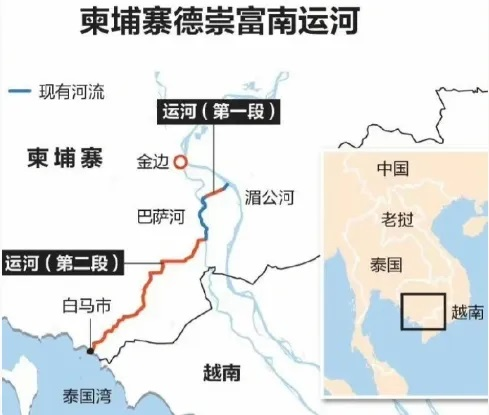
\includegraphics[width=9cm]{2024-08-17-001.jpg}
\end{figure}

\zd{简单一张示意图,任何人都能看出这条运河对柬埔寨的意义,对柬埔寨而言这条运河好处极大。}

\zd{但柬埔寨没有钱修这条运河,而且越南强烈反对。}

一带一路计划提出后,柬埔寨积极响应中国,修这条运河不管是技术难度还是钱对中国来说都是小菜一碟,所以在获得中国支持后,修这条运河不是问题了。

但越南反对,而且越南也是中国一带一路计划的重要成员国。

越南反对的理由很简单,因为这条运河对越南来说只有坏处没有好处。

本来每年躺赚的过路费没有了,利用出海口卡柬埔寨脖子的能力没有了。

而且一条河流的下游国家卡上游国家脖子这在全世界都是极其罕见的,正常来说都是上游国家卡下游国家脖子,哪怕是农村里两个村子争水源都知道肯定是上游占优势。

因为上游国家建造好水利设施后,只要愿意就可以随意控制水流,但下游国家修建再多水利设施都很难把水流给推回上游。

越南这么多年能利用出海口卡柬埔寨脖子,原因有两个,第一个是柬埔寨穷,第二个是柬埔寨打不过越南。

但如果中国牵头修建了德崇扶南运河,越南的武力优势就没有了,然后如果柬埔寨愿意,那这条运河作为一个巨大的水利设施,能让柬埔寨拥有反过来卡越南脖子的能力。

因此越南不同意这个计划。

中国提出了很多解决方案,比如让越南出钱入股,大家一起修这条运河,以后这条运河怎么用越南也有发言权,整个湄公河大家可以一起利用嘛,总归是把蛋糕做大了,至于利益分配好谈,这就是中柬越湄公河经济合作计划。

但越南对此毫无兴趣,做大湄公河流域蛋糕再分配利益这种事对越南没有吸引力,越南要的是就是不准修建这条运河,让自己可以一直卡柬埔寨脖子,至于其他的免谈。

这条运河完全修建在柬埔寨境内,属于绝对意义上的柬埔寨内政,修不修用得着你越南同意?

\zd{但越南上一任的一把手阮富仲很亲中,至少态度上很亲中。}

根据中国的一带一路计划,越南的胡志明港口为东南亚陆海交通的大动脉枢纽,东南亚铁路网里越南也是重要组成部分。

在阮富仲的任期内,虽然从实际结果来说什么都没落地,但从态度上来说阮富仲一直积极和中国谈判,把很多事情都谈到了看起来好像只差临门一脚的地步,而且比较注意保持和欧美的距离,面对美国宣称要把中国制造业转移到越南的诱惑也能保持微妙的端水平衡,还算安分,不像菲律宾那样傻愣愣的冲上去挑事。

所以我们还是比较考虑越南感受的,一直在和越南进行沟通协商,几年前这条运河的勘探工作就已经做好了,但一直没有开工修建,就是在等越南。

但给的时间周期是有限的,中国不会无限制的等越南。

而越南的执政人,也没有一直是阮富仲。

2024年7月19日,越南总书记阮富仲去世。

2024年7月25日,越南为阮富仲举行了国葬。

阮富仲走的很突然,没有安排好接班人,但最终越南还是选出了自己的最高领导人,苏林。

这个人不算亲美派,但绝对不是亲中派,其长期以来的政治宗旨是在中美之间反复横跳,借此为越南博取利益,一直拖着东南亚铁路计划,拉日本入局施压中国,想一分钱不出让中国出人出钱出技术修高铁思路的提出者就是苏林。

成为越南新领袖后,苏林还是这个思路。

7月31日,越南中央理论委员会主席阮春胜率领代表团,对美国进行访问。

8月3日,苏林宣誓就职。

8月4日,阮春胜带着代表团从美国返回越南。

越南新政府上台后第一个访问的不是中国,甚至不是俄罗斯,而是美国。

但去的人并不是最高领袖苏林,而是中央理论委员会主席阮春胜,还是在苏林宣誓就职前去的。

这政治小把戏耍的,以为自己是擦边球高手。

毫无疑问,如果越南做出这种行为没有任何代价,甚至还能捞到好处,那未来苏林任期内整个越南必然是在中美之间反复横跳,时不时的就给中国找麻烦。

至于一带一路计划,那是绝对不可能配合中国落地的,想都别想。

\zd{因此在7月31日阮春胜带着越南代表团落地美国之后,中国在8月1日联合柬埔寨宣布德崇扶南运河工程正式启动。}

越南不想谈那就别谈了,不想要入股拿话语权和利益分配权,那就别要了。

8月4日阮春胜带着越南代表团带着越南代表团从美国返回。

\zd{8月5日当天,柬埔寨德崇扶南运河正式开工,柬埔寨首相携夫人以及2万人参加开工典礼,同时柬埔寨全国当日放假一天,举国为德崇扶南运河工程的开工进行庆祝。}

这时间点卡的,就是卡给越南看的。

\begin{figure}[H]
    \centering
    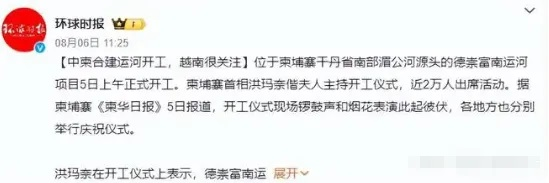
\includegraphics[width=9cm]{2024-08-17-002.jpg}
\end{figure}

德崇扶南运河正式动工的这一刻,谁都拦不住这条运河的建成了,至于这条运河怎么修,修成什么样,只有中国和柬埔寨有权决定,无需考虑其他任何国家的意见,因为运河股东方只有中国和柬埔寨。

\zd{这时候越南和柬埔寨的谈判关系就强弱颠倒了,因为这条运河对柬埔寨而言只是经济发展的问题,但对于越南而言则不止是经济发展的问题。}

整个地球都是上游可以卡下游脖子,没有例外,以前越南和柬埔寨的关系只是特例。

对柬埔寨而言,这条运河挖深一米或者加宽1米,那只是多费点成本而已,但对于越南来说就不一样了。

平时还好,但遇到旱季或者洪水,因为运河的掌控权在柬埔寨手中,越南一股都没有,所以怎么分配运河的水量到时候就只能越南来求柬埔寨配合了。

湄公河下游的湄公河三角洲是个风水宝地,罕见的天地粮仓,稻米2年7熟,整个越南56%的粮食产量都来自于湄公河三角洲。

\begin{figure}[H]
    \centering
    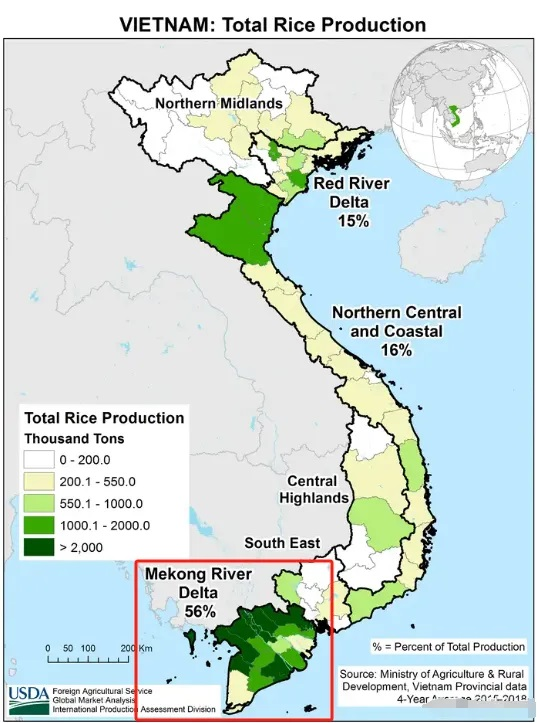
\includegraphics[width=9cm]{2024-08-17-003.jpg}
\end{figure}

风调雨顺那就罢了,但如果碰到旱情,运河水位严重下降到不足以支撑通航的地步了,那柬埔寨是让整条运河停航,中断柬埔寨的物流运输和经济发展来保证越南的粮食产量,还是截留本就不足的河水来保证柬埔寨的运河通航能力?

运河越宽,这种截流能力越强,虽然费钱但也能提升运河的通行能力。

如果这个运河修建的足够宽,那在极端天气情况下甚至有能力让湄公河改道,海水倒灌,湄公河三角洲盐碱化。

但反过来,如果碰上洪灾,大量的洪水奔流而下,湄公河三角洲的粮食产量和人口会遇到严重威胁,这个时候只要柬埔寨愿意付出“小小代价”,就可以强行拦截水流蓄在柬埔寨的运河里,只是淹没一些运河沿岸的柬埔寨民居而已,但可以保护整个湄公河三角洲。

但柬埔寨凭什么牺牲本国的一些民居?哪怕可以保护整个湄公河三角洲,柬埔寨没有牺牲自己保护越南的义务。

而且运河越深,这种蓄洪保护能力就越强,但特别费钱,比加宽费钱的多,因为加深需要修建岸上堤坝,而这种费钱对柬埔寨来说没什么好处,运河挖浅一点,够用就行,碰到洪水了打开所有水坝开关,一股脑全扔给下游是最省钱的。

所以运河怎么修,宽深怎么定,平时运营的时候碰到旱灾和洪灾怎么对下游分配水量,越南是非常有必要参与的,充分吸取越南意见,并让越南承担多出来的成本,对越南是最有利的。

\zd{但越南既然不愿意参与,那就别参与了。}

这条运河修多宽多深,以后水量怎么分配,和越南一毛钱关系都没有,有特殊要求就过来求,求一次柬埔寨就酌情办一次,不求那日常经营,也就是每天开闸放水的量,当然是柬埔寨自行决定。

不知道为什么越南没有考虑过中国撇开越南和柬埔寨单独修建运河的可能性,要知道这条运河完全在柬埔寨境内,修建根本不需要越南进行任何配合,\zd{之前找越南协商那只是出于情谊和把事情做圆满的心态,不是说必须得到越南同意。}

但当真的把越南撇开后,整个越南都慌了,自家上游修建这么大一个水利工程,还掌控在柬埔寨手中,未来什么后果猜都猜得到,因为自己这么多年是怎么利用湄公河卡柬埔寨脖子的越南人记得可是很清楚。

从不利用上游优势卡下游脖子的国家全球仅中国一家,中国对东南亚那样巨大的上游优势如果是欧美国家掌控,早就把下游国家拿捏的嗷嗷叫了,手段简直不要太多。

什么旱期蓄水洪期排水,什么把下游变成小型恒河,每一种都是能把下游搞的苦不堪言但拿上游没办法的。

欧美不是中国这样的国家,但越南和柬埔寨也不是,所以越南很怕自己被柬埔寨卡脖子。

这几天的网上可热闹了,越南网友和柬埔寨网友在网上激情对骂。

\zd{越南网友的大意就是打算以实力的地位和柬埔寨对话,而柬埔寨网友的大意就是你们有个屁的实力。}

因为中国早就提前杜绝了这种越南以实力阻止运河修建的可能性。

2024年,中国和柬埔寨举行了联合军演。

\begin{figure}[H]
    \centering
    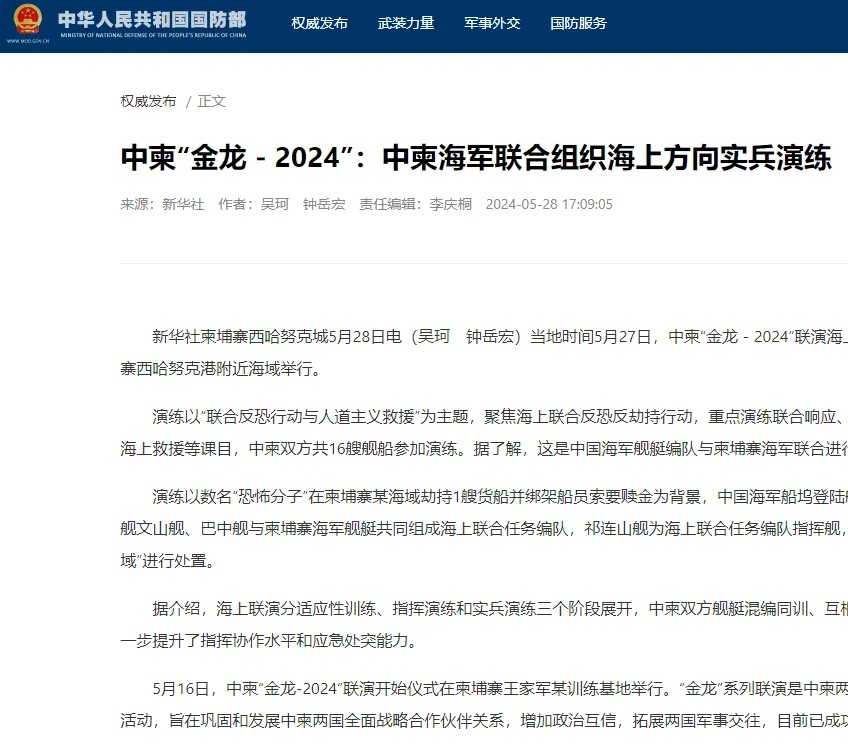
\includegraphics[width=9cm]{2024-08-17-004.jpg}
\end{figure}

你猜好好的,中国为啥要和柬埔寨举行联合军演?

2024年,柬埔寨进行了大阅兵,向世界展示了全套中式机械化部队。

\begin{figure}[H]
    \centering
    
\includegraphics[width=9cm]{2024-08-17-005.jpg}
\end{figure}

不仅全军都是中式武器,而且整个部队的机械化装备都是采购自中国。

\zd{而中国的两艘056A,从去年12月开始就一直停在柬埔寨云壤海军基地了,到今天已经停留了足足8个月没动。}

\zd{做这些事,就是为了让柬埔寨可以和平发展本国经济。}

越南网友想“以实力地位解决问题”?

如果发生了这种事,那。。。


\yh{
    汉兵方至,毋敢动,动,灭国矣
    \begin{flushright} ——汉使傅介子 \end{flushright}
}

今年7月6日,中国外交部发言人汪文斌调任柬埔寨大使。

\begin{figure}[H]
    \centering
    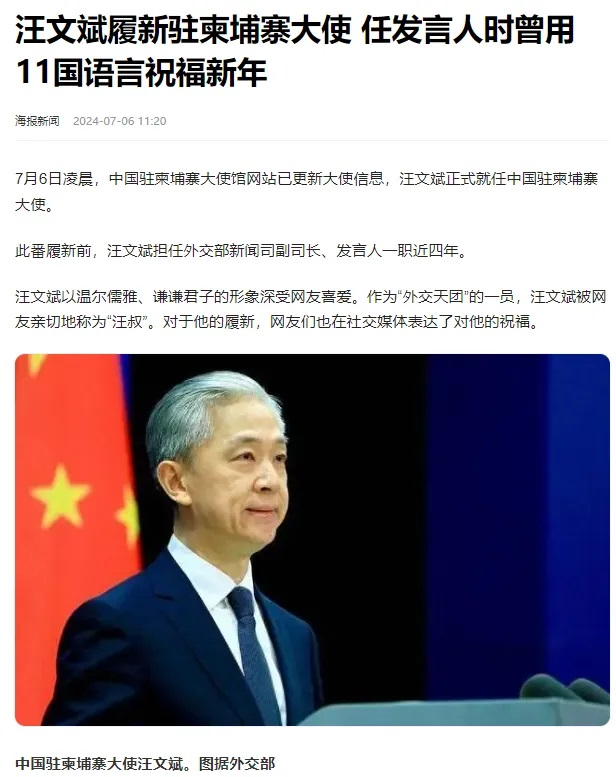
\includegraphics[width=9cm]{2024-08-17-006.jpg}
\end{figure}

汪文斌这么高级别的外交部人员为什么会调到一个小小的柬埔寨当大使?一个月前很多人看到这个新闻都很迷惑。

\zd{一个月后答案揭晓,这哪是去柬埔寨当大使啊,这是去柬埔寨履职安南都护了。}

越南这些年对一带一路计划阳奉阴违,早就到了我国能容忍的临界点,我国最近一年的做法就是逼越南表态,一带一路计划到底搞不搞必须给个说法,不允许再拖了。

最后越南表态了,不搞,派使团出访美国去了,准备继续骑墙捞好处。

表态第二天,柬埔寨德崇扶南运河工程就启动了。

巴不得你越南这么表态,拉越南谈这个运河本来就很麻烦,正好趁这个机会撇开越南直接开建形成既有事实,顺便借越南这个机会杀鸡儆猴。

\zd{因为一带一路的关键枢纽工程可不止德崇扶南运河这一个,我国的一带一路工程不是单纯的给东南亚穷国搞基建形成一体化经济圈,而是一牌多用,凭空增大自己的政治筹码。}

根据中国公布的一带一路计划,德崇扶南运河的下一个枢纽也是个运河,叫泰国克拉运河,完全在泰国境内。

这个计划简单的说就是把泰国的克拉地峡给凿穿,在马六甲海峡之外生生的造出第二条海运枢纽,大幅减少通往中东地区的航程,且避免了马六甲海峡这条海运枢纽没有掌握在中国海军手中的潜在风险。

\begin{figure}[H]
    \centering
    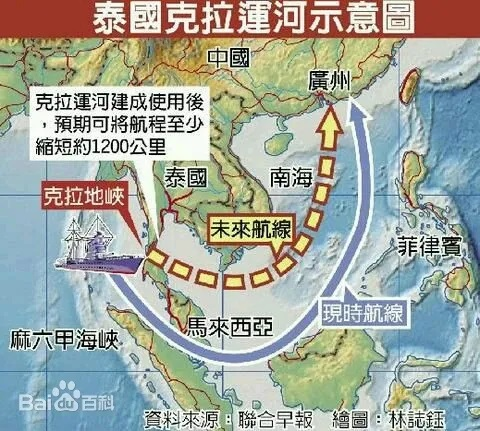
\includegraphics[width=9cm]{2024-08-17-007.jpg}
\end{figure}

根据一带一路的总规划图,未来不止上海广东的海船可以直接走克拉运河,中国大西南还有整个东南亚地区的货流,都可以通过铁路和德崇扶南运河集中到柬埔寨的海港中,装船后进行运输。

\begin{figure}[H]
    \centering
    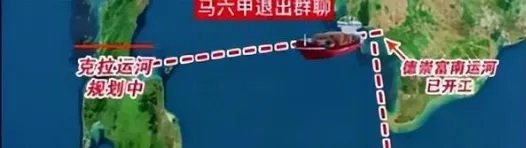
\includegraphics[width=9cm]{2024-08-17-008.jpg}
\end{figure}

所以德崇扶南运河一旦建成,需要运输的远不止目前柬埔寨自己境内的那点货,整个中国西南和东南亚的工商业产品都会向这里调配。

修建克拉运河对中国好处极其巨大,以后中国的海船想走马六甲海峡就走马六甲海峡,想走克拉运河就走克拉运河,避免了马六甲海峡物流被人截断的潜在风险,甚至中国海船走克拉运河还更省运费。

修建克拉运河对泰国而言好处也极其巨大,这等于凭空给泰国造了一棵摇钱树,新加坡依靠马六甲海峡过的有多爽,未来的泰国依靠克拉运河过的就能有多爽。

但对于修建克拉运河,泰国没钱没技术,只能依靠中国,所以泰国最近几年极其亲华,对一带一路计划极其配合。

而修建克拉运河有一个绝对的受害者,那就是新加坡,如果克拉运河建成,那原本停靠新加坡港口的海船至少会被克拉运河分走一半,甚至更多。

所以新加坡肯定反对克拉运河计划,但克拉运河是建在泰国境内,中国出钱出技术,和上千公里之外的新加坡一毛钱关系都没有,世界上也从来没有你垄断了某个海峡的运输就不准别国建运河这种说法。

所以新加坡无力反对克拉运河的修建,而克拉运河对中国的作用不仅是减少那点航程和运费,更关键的是解除了马六甲海峡被切断给中国带来的安全风险。

因此中国是肯定要修建克拉运河的,但新加坡也是一带一路计划的成员国,中国需要考虑新加坡的感受。

虽然在泰国修克拉运河和新加坡没啥关系,但面子上会给足新加坡。

而新加坡选择的应对办法和越南截然不同,新加坡这几年很亲华,非常亲华,不仅全方位的支持中国,甚至在公开场合反复讽刺和批评欧美,给中国强站台。

\zd{每个月新加坡都会派出一名高级官员从某一个角度,在讲座或者电视节目中骂一次欧美,注意频率已经达到了每个月都要骂一次,相关新闻铺天盖地。}

\begin{figure}[H]
    \centering
    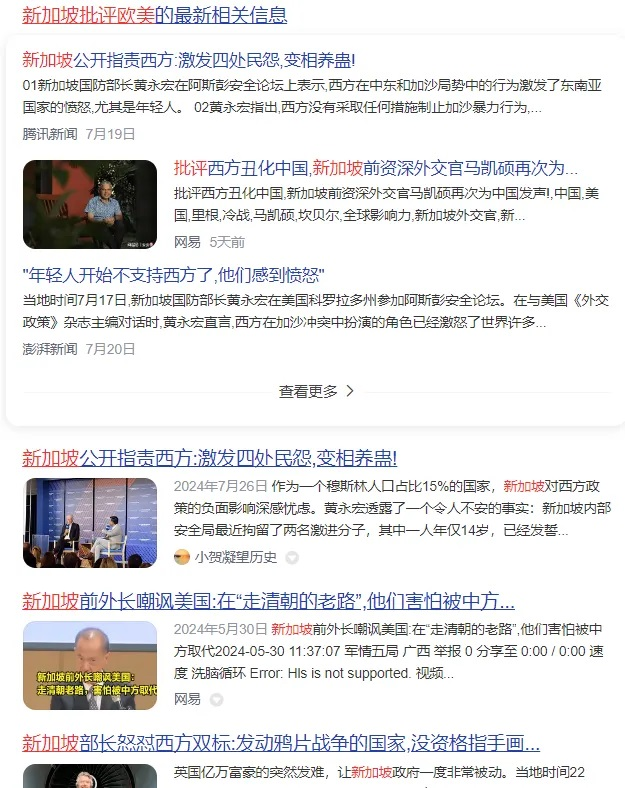
\includegraphics[width=9cm]{2024-08-17-009.jpg}
\end{figure}

新加坡这么给面子,那这个克拉运河当然就不好意思修建了。

而且新加坡如果愿意沿着亲华的路一直走下去,未来采取某种方式让中国对马六甲海峡具有安全感,那克拉运河也可以不修建,毕竟中国不介意钱是被新加坡赚了还是泰国赚了,要的只是安全感。

\zd{不说让中国海军基地入驻马六甲海峡,至少要把美国海军基地从马六甲海峡赶走。}

撇开越南直接修建德崇扶南运河,不止是修给越南看的,也是修给新加坡看的。

如果一直亲华,那一切好谈,大家的面子和利益中国都会考虑到。

\zd{如果反华或者当骑墙派,那就不好意思了,修这些运河本来就是别国内政,本来就无需考虑其他国家的意见,拉你过来谈是给面子,不拉你过来谈才是本分。}

这个就是阳谋,中国没有给越南和新加坡任何好处,而且一带一路计划也确实是造富所有人,增大所有沿线国家蛋糕的好计划,都配合的话所有人都有增量蛋糕吃。

但利用一带一路计划里的关键枢纽,我们达到了虚空造牌的效果,不花钱就把事办了。

我们也没对越南怎么样,和柬埔寨修个德崇扶南运河,就让越南觉得自己好像“被惩罚”了,但实际上我们根本没有搭理越南,彻底绝对的不干涉越南内政。

未来如果和泰国修建克拉运河,那同样也是和新加坡无关,隔着上千公里呢关你什么事。

\zd{但利用这纸上的计划,以前一贯在东西方骑墙捞好处的新加坡,就被迫改变了自己的外交路线,从骑墙变成了单方面亲华。}

但我们既没有逼迫新加坡什么,也没有给新加坡好处,甚至提出的一带一路计划无论你怎么看都是造福东南亚国家,甚至是造福全人类的好计划。

\zd{给穷苦落后国家修路修桥修运河,有问题?}

书本上教的地缘政治学,说的是如果外交结果没有朝着有利于你的方向去发展,那你就需要以地缘因素作为第一考量,修正你的外交策略。

\zd{但中国发明了另一种地缘政治学,那就是如果外交结果没有朝着有利于自己的方向去发展,那我们就直接修改地缘因素。}

\zd{没办法,我们的工程队拥有地图编辑器。}

这次的柬埔寨德崇扶南运河,直接修改了整个柬埔寨以及上下游国家的物流、人流以及财富分配方向,和施工中的东南亚铁路网结合后,大幅改变了东南亚的地缘格局。

而这样的工程枢纽,在一带一路计划中还有好多个,远不止隔壁泰国的那个克拉运河,中国在所有关键地缘节点都有对应布局。

利用这些布局带来的地缘利益改变,这些布局的周边国家逐渐走上亲华之路,无论是否自愿都会逐渐变得亲华,因为地缘利益使然。

\zd{中国的布局不是单纯的搞基建送温暖,考虑极多,很多布局落地有好处,不落地那也有好处,虽然最终都肯定落地,但在没落地的谈判过程中,也能给中国带来巨大的政治好处。}

无论沿线国家听话还是不听话,配合还是不配合,中国都预备了对应手段,而且是光明磊落的手段,毕竟我们做的事是增大所有人蛋糕,是阳谋,任你怎么挑刺都说不出个不是。

这次柬埔寨德崇扶南运河在8月5日正式开工后,刚带使团从美国回来的越南估计找美国协调沟通了,希望美国帮忙解决此事,但美国能做的只是出动舆论工具,发几篇文章从环保方面搞点小麻烦而已,其他的什么也没做。

8月8日,越南放弃了挣扎,认清了现实,明白这条运河是非建不可了,于是越南外交部副发言人段克越在例行记者会上表态说:

\yh{ “湄公河是越南、老挝和柬埔寨三国的宝贵财富,是三国团结精神和特别友谊的交汇之地。越南希望同包括柬埔寨在内的湄公河沿岸国家一起合作,有效和可持续管理湄公河水资源,造福湄公河沿岸居住的居民,致力于子孙后代的未来和沿岸国家之间的密切团结。”}

给大家翻译一下,越南的意思就是大家一直以来都是好朋友,希望柬埔寨以后在调配运河水量的时候考虑下越南,大家要合作,要团结,不要对抗。

\zd{你看,越南要开始和柬埔寨谈合作和团结了,早干嘛呢。}

\zd{但是,不然越南还能怎么办呢,等运河建好了,那开关是真的掌握在柬埔寨人手里的。}

当初制定一带一路计划的时候就已经考虑了所有可能性,越南如果跳反怎么应对早就被写入应对方案了,我们这个计划是大型国家战略,这种长达一二十年的国家战略从来不考虑靠投机取巧以及靠意外成功的这种可能性,只做阳谋,无论任何情况都必然成功的那种阳谋,依靠国力和堂堂正正之势逐步落实计划。

不知道越南是哪来的信心去搞小动作的,让自己凭空被剥离了一部分控制权,以后这条运河的事情越南只能求柬埔寨配合了。

\zd{小阴谋,对抗不了大阳谋,只会给自己带来损失。}

\end{document}

